\begin{enumerate}
	\item A solid cylinder of 10cm diameter and 40 cm long consists of two parts made of different materials. The first part of the base is 1.0cm long and of specific gravity = 6.0. The other part of the cylinder is made of the material having a specific gravity of 0.6 as shown in Figure 1. Determine if it can float vertically in water. \marks{10}
	\begin{figure}[h!]
		\centering
		\label{figa1}
		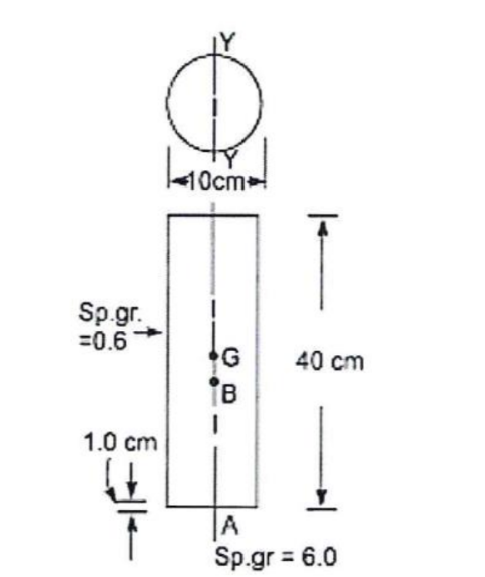
\includegraphics[width=80mm]{fm.png}
		\caption{Diagram for use}
	\end{figure}
\newpage
\item Evaluate the following limits
\begin{enumerate}[(i)]
	\item $\lim\limits_{x\rightarrow 0}$ $\dfrac{\sin x}{2x}$ \marks{3}
	\vspace{0.2cm}
	\item $\lim\limits_{x\rightarrow \infty}$ $\dfrac{8x^{3} - 9x -1}{-12x^{3}+1}$ \marks{3}
\end{enumerate}
\item For what values of the constant K is the function continuous for all values of $X$\marks{3}
\begin{equation*}
	f(x) = 
	\begin{dcases}
		KX + 5 &  X < 1  \\[1ex]
		x^{2}-3x + 4 & X \geq 1 
	\end{dcases}
\end{equation*}
\item Determine whether the series $\displaystyle{\sum_{n=1}^{\infty}}\frac{n}{n+1}$ converges or diverges. \marks{3}
\end{enumerate}